% Workshop handout — special-lab-1: J-space replication on OLMo-3-32B-Think
% Compile: pdflatex (twice). Figures in ./figures/.
\documentclass[10pt]{article}
\usepackage{lmodern}
\usepackage[T1]{fontenc}
\usepackage[margin=2.2cm]{geometry}
\usepackage{graphicx}
\usepackage{booktabs}
\usepackage{multirow}
\usepackage{microtype}
\usepackage[hidelinks]{hyperref}
\usepackage{xcolor}
\graphicspath{{figures/}}

\newcommand{\jlens}{\texttt{jlens}}
\newcommand{\code}[1]{\texttt{#1}}

\title{\bfseries The J-space in OLMo-3-32B-Think:\\
\large an open-weights replication of ``Verbalizable Representations Form a
Global Workspace in Language Models''}
\author{special-lab-1, interpretability labs% <-- replace with author name(s)
}
\date{July 26, 2026 \\[2pt] \small run \code{2026-07-25\_1726} \;\(\cdot\)\;
lens \jlens{} @ \code{581d3986} \;\(\cdot\)\; seeds 0 \\[2pt]
\small\color{gray!60!black} v2 delta run in progress (\S\ref{sec:v2}):
results below marked [v2] update as instruments land}

\begin{document}
\maketitle

\begin{abstract}
\noindent
We replicate the core claims of Anthropic's July 2026 ``global workspace''
paper on \textbf{Olmo-3-32B-Think}, a fully open (weights + training data)
reasoning model, using the reference Jacobian-lens implementation. The
\emph{geometry} replicates: a sparse, verbalizable subspace concentrated in
the middle layers, whose directions are read by 73--94 downstream components
(vs.\ 0 for random directions). Its \emph{capacity} is roughly an order of
magnitude thinner than reported for Claude ($\le$0.67\% of activation
variance vs.\ 6--10\%; $\sim$6 active concepts vs.\ $\sim$25). The paper's
headline \emph{causal dissociation does not replicate} at our doses: static
J-space ablation is indistinguishable from random controls, while
matched-dimension \emph{non-verbalizable} high-variance directions cause the
real selective damage. Exploiting the thinking variant, we add a result the
paper could not test: the workspace does \emph{not} contain the answer before
reasoning begins (median rank 5613), but \textbf{leads the chain of thought by
a median 46 tokens} during reasoning, and is loaded on demand when thinking is
suppressed (rank 211 at the answer position, collapsing monotonically
L30$\to$L60). An eval-awareness probe finds a highly consistent
``being-evaluated'' readout direction ($p<10^{-3}$ on all probed layers) that
is semantically legible yet behaviorally inert under ablation.
\end{abstract}

\section{Setup}

\textbf{Model.} \code{allenai/Olmo-3-32B-Think} (64 layers, $d=5120$), bf16 on
one 96\,GB RTX PRO 6000 Blackwell --- full-precision tier: no quantization, no
gradient checkpointing.
\textbf{Lens.} Reference \jlens{} package (\code{anthropics/jacobian-lens}),
fit on 120 WikiText-103 prompts $\times$ 128 tokens (the neuronpedia reference
recipe; \jlens{} README reports saturation near 100; the paper used 1000).
Source layers: dense middle band L20--44 (step 2) + early/late controls
\{4,8,12,16,48,52,56,60\}; target L63; four 30-prompt slices merged via
\code{JacobianLens.merge}. Fit cost 5.2\,h ($\sim$157\,s/prompt, peak
80.6\,GB); per-prompt $\max\|J\|/\sqrt{d}$ stable at 0.94--0.95 and
running-mean deltas fell $\sim 1/n$ (converged).
\textbf{Dictionary.} Concept $i$ at layer $\ell$ read through the
RMSNorm-gain linearization $(W_U \odot g)\,J_\ell$, rows normalized.
\textbf{Sanity gate.} Easy single-token factual probes: 17/21 hit rank
$\le$20 mid-band for \emph{both} J-lens and logit lens (ceiling). The
discriminative check, multihop bridge-entity readout at the final prompt token
($n=60$): J-lens pass@1 \textbf{0.283} vs.\ logit-lens 0.200 (+41\% rel.);
pass@20 0.547 vs.\ 0.586 --- J-lens sharpens the rank-1 readout without
expanding the top-20 shortlist, the same ``replicates, less clean'' flavor as
Nanda's Qwen~3.6~27B replication.

\section{How to read the instruments (reader's model)}

Three orientation points carry every result below; the full version with
worked examples is \code{report/REPORT\_v2.md} \S``How to read this lab''.

\textbf{(1) The lens is a fitted, averaged Jacobian.} $J_\ell = \partial
\text{logits}/\partial h(\ell)$ --- all downstream layers collapsed into
one linear map --- estimated \emph{once} over the fitting corpus and
frozen; readout is a matrix multiply, no per-prompt backprop. Dictionary
row $v$ is a \emph{push} direction (``moving $h(\ell)$ this way most
raises token $v$'s final logit''), not output-space resemblance --- which
is why a concept can be J-visible while logit-lens-invisible if its
coordinates only become output-aligned many layers later, and why the
J-advantage lives in the mid band. One linearization for all inputs is
also the method's noise source (and why the fitting corpus is a real
degree of freedom). \textbf{(2) The readout claim is not the workspace
claim.} Finding the hidden bridge --- item 0: \emph{``the language spoken
in the country where the Amazon River ends''} $\to$ Brazil (never
stated) $\to$ \emph{Portuguese} --- makes a better logit lens. The
workspace claim is a \emph{conjunction}: small $+$ localized $+$
broadcast $+$ \textbf{causally privileged}. This lab tests the
conjunction; it breaks at the causal joint. \textbf{(3) Read causal
cells with the prior inverted.} Each ablation removes $<$1\% of
dimensions carrying a measured $\approx$0.5--1.1\% of activation energy
--- the default expectation is \emph{nothing happens}, and the
energy-matched random control delivers exactly that. In database terms:
\emph{static span} drops one small shared temp-table (same directions
for every prompt) --- only the dissociation pattern ``multi-join queries
fail, single-table lookups survive, fluency survives'' would count as a
workspace, and that pattern never appears on either model;
\emph{frozen per-item} deletes the row (rank the dictionary on the
item's prompt, freeze top-10) --- its headline is expected, its value is
the conjunction (a linear projection sufficed; the random-dictionary
twin does nothing; \emph{amnesia not aphasia} --- generations stay
coherent; and the 1-hop/2-hop damage shape classifies content-vs-
scratchpad); \emph{live per-token} re-selects each step and so deletes
each word as it is born --- maximally dramatic, minimally informative
(the community replication's confound, here measured with a matched-live
control). If ``deleting key ideas breaks output'' feels unsurprising:
correct --- that instinct, formalized with controls, is the analysis.
The paper needed the \emph{unexpected} pattern; both models delivered
the expected one, so the earned label is \emph{content channel} (with
the P5 rescue and Qwen's spared one-hop as the two epilogues that keep
it interesting).

\section{Descriptive geometry: the workspace exists, ten times thinner}

Sparse nonnegative gradient-pursuit decomposition of 200 diverse prompts
(factual QA, chained arithmetic, code/SQL, prose) onto the dictionary:

\begin{itemize}\itemsep2pt
\item \textbf{Sparsity.} Median active concepts per (position, layer):
\textbf{6} at $\theta{=}0.01$, 3 at $\theta{=}0.02$, $k_{90}\!\approx\!4$,
peaking at L36--42. Paper: $\sim$10--25.
\item \textbf{Variance share.} $\le$\textbf{0.67\%} of centered activation
variance inside the band (0.91\% at L60, unembedding-adjacent). Paper:
6--10\%. The capacity gap ($\sim$10$\times$) is threshold-robust.
\item \textbf{Localization.} The cleanest signature is top-1 persistence
across adjacent positions: 0.19--0.20 at L32--40 vs.\ 0.03--0.08 at both ends
--- an inverted U at 50--66\% depth (paper band: 33--92\%).
\item \textbf{Broadcast --- with a catch.} Top J-directions at L24/32/40 are
read (input-projection alignment $z>3$) by \textbf{73--94} downstream
components vs.\ \textbf{0} for matched random directions ($p\approx10^{-24}$).
But matched-dimension top \emph{non-J} principal components are read by
77--125: wide readout is a property of high-variance directions generally,
not of verbalizable ones specifically.
\end{itemize}

\begin{figure}[htbp]
\centering
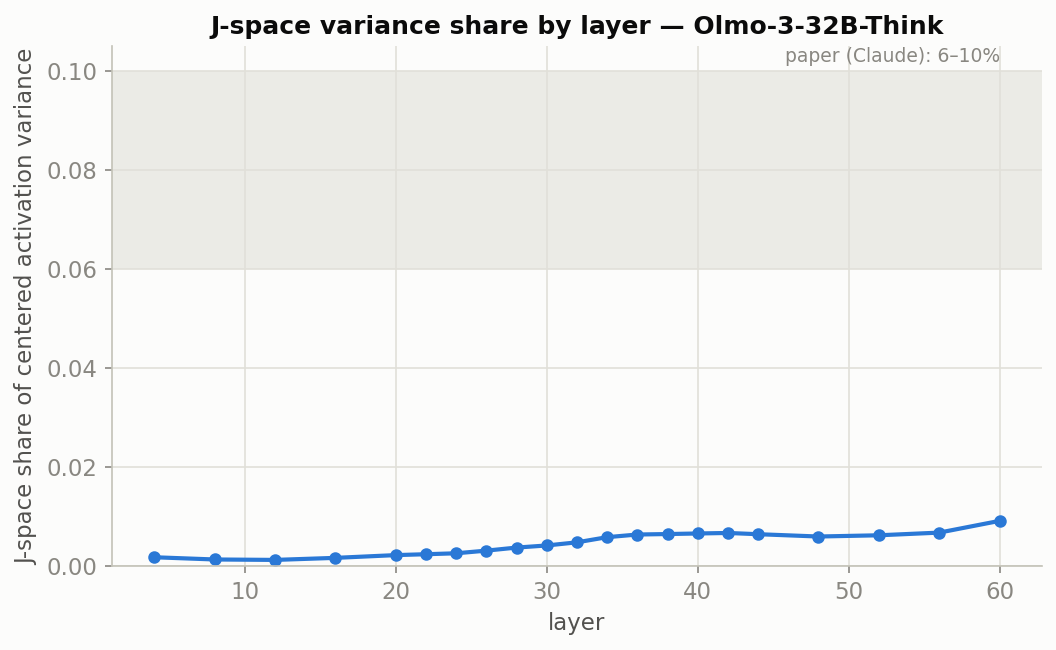
\includegraphics[width=.48\linewidth]{f1_variance_share_by_layer.png}\hfill
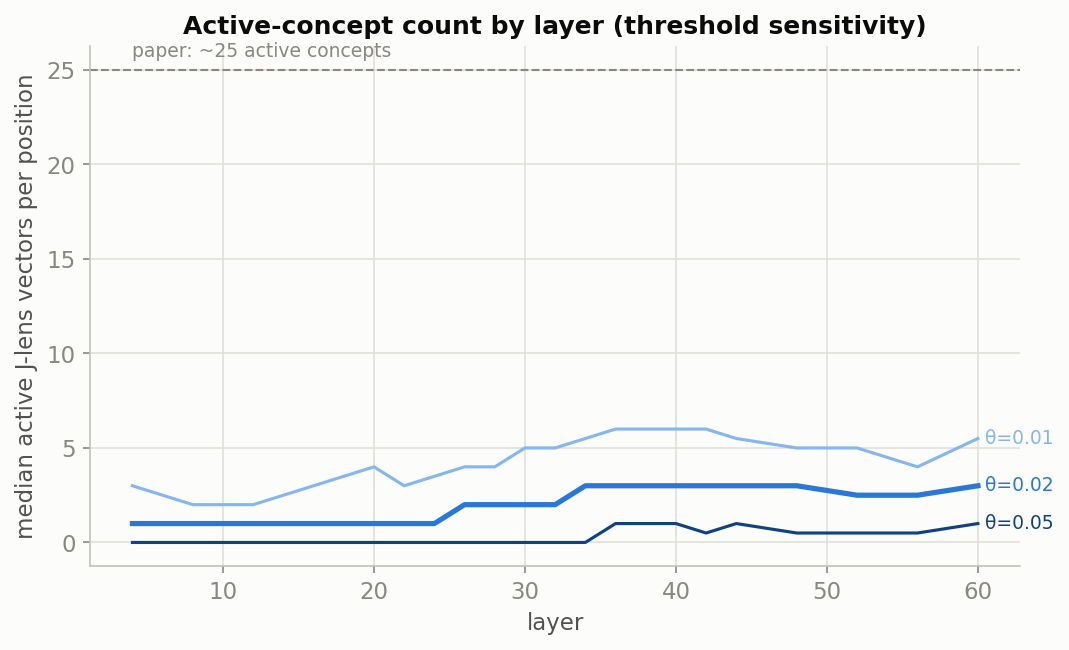
\includegraphics[width=.48\linewidth]{f2_active_concepts_by_layer.png}
\caption{\textbf{Left:} J-space share of activation variance by layer; shaded
band = paper's Claude range (6--10\%). \textbf{Right:} median active-concept
count by layer under three activation thresholds; dashed line = paper's
$\sim$25.}
\end{figure}

\section{Causal ablation: the dissociation does not replicate}

Battery: 2-hop probe-swap facts ($n{=}60$), chained arithmetic ($n{=}30$),
3-table SQL with join-key checks ($n{=}30$), vs.\ one-hop facts, grammatical
minimal pairs, held-out prose NLL. Conditions (band L20--44, doses
$k\in\{10,20,40\}$ dims/layer, 2000-resample bootstrap CIs): static top-$k$
J-span; matched random subspace; matched top non-J PCs; paper-faithful
per-token dynamic top-10.

\begin{table}[htbp]
\centering\small
\begin{tabular}{lccccccc}
\toprule
condition & 2-hop & 2-hop $\Delta$lp & arith & SQL & 1-hop & grammar & NLL \\
\midrule
none (baseline)        & 0.58 & ---            & 0.87 & 0.67 & 0.60 & 1.00 & 2.71 \\
J-space dyn top-10     & 0.00 & $-$23.0        & 0.00 & 0.00 & 0.00 & 0.30 & 24.34 \\
J-span $k{=}20$        & 0.52 & $-$0.17        & 0.93 & 0.67 & 0.60 & 1.00 & 2.85 \\
random $k{=}20$        & 0.52 & $-$0.08        & 0.90 & 0.67 & 0.60 & 1.00 & 2.75 \\
non-J PCA $k{=}20$     & 0.28 & $\mathbf{-0.86}$ & 1.00 & \textbf{0.00} & 0.70 & 1.00 & 3.45 \\
\bottomrule
\end{tabular}
\caption{Accuracy (and 2-hop answer-logprob delta vs.\ baseline) under
ablation; $k{=}10/40$ follow the same pattern. Static J-span $\approx$ random
everywhere; the \emph{non-verbalizable} control causes the selective damage.}
\end{table}

Three observations. (1) The paper-faithful \emph{dynamic} condition removes
whatever the model is currently computing --- output degenerates to asterisks,
NLL 2.71$\to$24.34 --- reproducing the ``live-computation confound'' Nanda
flagged; it cannot count as evidence for a workspace. (2) Static J-span
ablation is statistically indistinguishable from random subspaces on every
task \emph{and} on the finer answer-logprob instrument
($\Delta$ $-0.15\ldots-0.18$ vs.\ $-0.01\ldots-0.11$; CIs straddle 0).
(3) The non-J high-variance control produces the only structured damage ---
and generation samples show its signature is \emph{register destruction}: SQL
completions lose the formal register entirely (\code{SELECT the user's city
and the user's country, and the user's name, \ldots}) while arithmetic
content survives. At these doses, OLMo's causal load sits in generic
high-variance directions, not in the verbalizable subspace.

\begin{figure}[htbp]
\centering
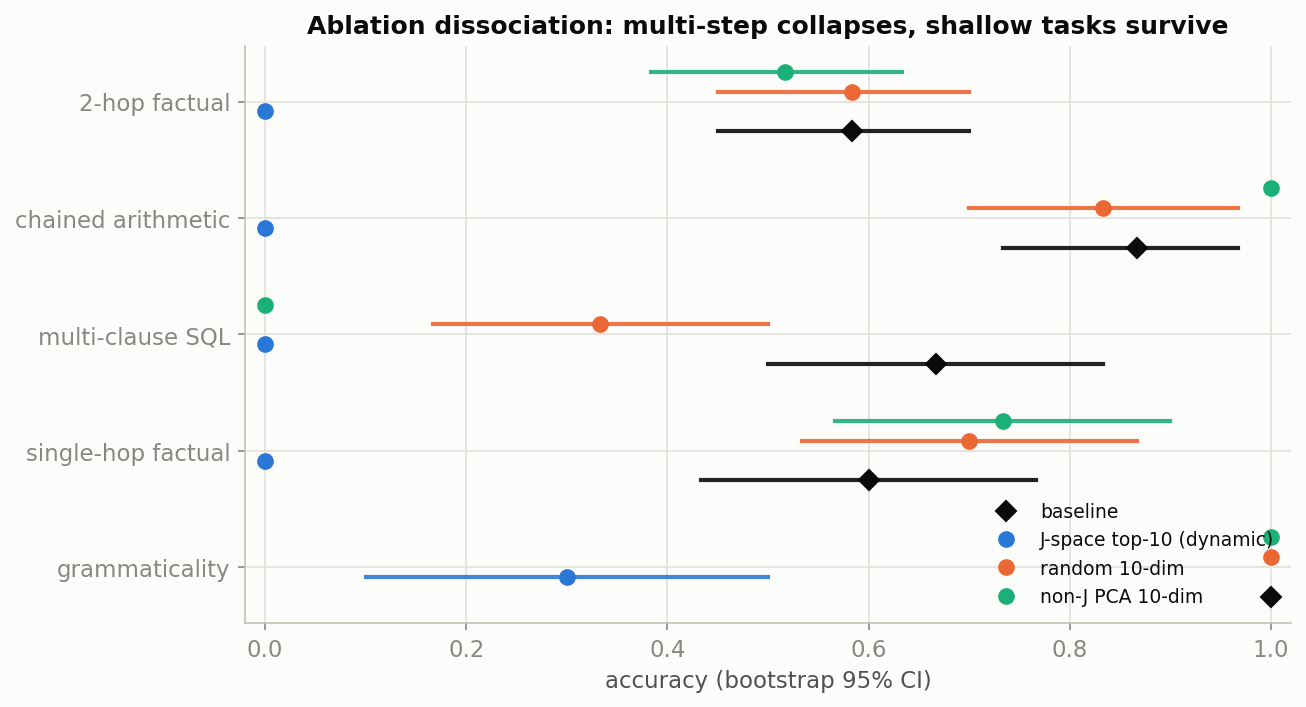
\includegraphics[width=.48\linewidth]{f4_ablation_dissociation.png}\hfill
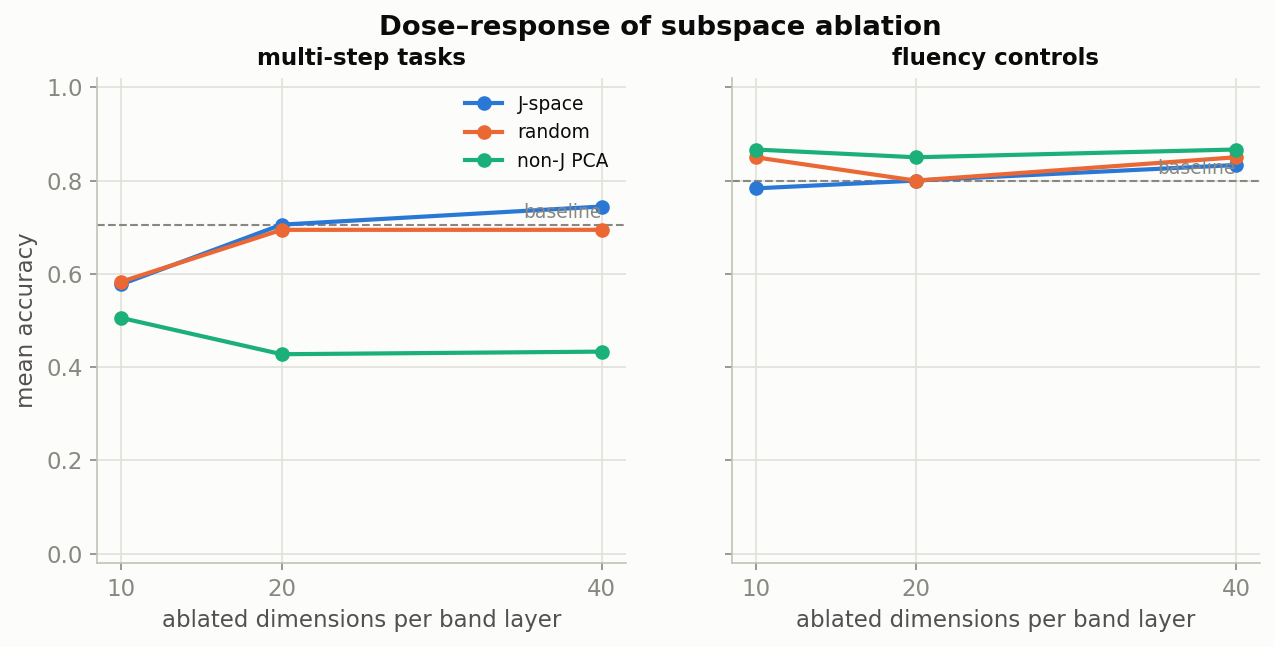
\includegraphics[width=.48\linewidth]{f5_dose_response.png}
\caption{\textbf{Left:} per-task accuracy with 95\% bootstrap CIs under the
$k{=}10$ conditions. \textbf{Right:} dose--response for multi-step vs.\
fluency task groups.}
\end{figure}

\section{The thinking-model angle: the workspace leads the chain of thought}

Olmo-3-32B-Think emits explicit reasoning tokens, so the paper's identity
claim (workspace content $=$ verbalizable reasoning substrate) becomes
testable in time. 90 items (40 two-hop, 30 chained arithmetic, 20 SQL
join-key); J-readout at L24/32/40 at every generation step; suppressed-CoT
variant closes the template's open \code{<think>} immediately.

\begin{itemize}\itemsep2pt
\item \textbf{Pre-CoT anticipation: null.} At the final prompt token the
answer's median J-rank is \textbf{5613} (10\% of items $\le$20); logit lens
11610 (0\%). The workspace does not precompute the answer before reasoning.
\item \textbf{Intra-CoT anticipation: strong.} The answer enters a read
layer's top-8 during thinking in 82--100\% of items, and on traced items
($n{=}34$) the workspace holds the answer a \textbf{median 46 steps before
the CoT first states it} (2-hop 48.5, SQL 38, arithmetic 9.5; workspace first
in 91\% of items).
\item \textbf{Answer-time loading.} Forcing an immediate answer (closed
\code{</think>}, zero reasoning tokens) pulls the answer's median rank from
5613 to \textbf{211} (23\% $\le$20), collapsing monotonically
L30$\to$L60: $2048 \to 1549 \to 519 \to 305 \to 118 \to 63 \to 10 \to 6$,
with J-lens ahead of logit lens through L28--40. Suppression costs accuracy:
2-hop $0.95\to0.82$, arithmetic $1.00\to0.90$, SQL $1.00\to1.00$.
\item \textbf{Faithfulness probe.} 116 events where a stable workspace top-1
word never appears in the nearby CoT (59/90 items) --- but only 4 involve the
final answer. The recurring divergent words are \emph{discourse-mode}
adverbs: \code{famously} (stable top-1 for 7--10 steps while the CoT recalls
``Springfield \ldots{} birthplace of basketball''), \code{respectively},
\code{etc} during enumerations. We find no ``workspace holds X, CoT argues Y,
answer is X'' case; the workspace appears to track the discourse mode of the
current reasoning span rather than concealed content.
\end{itemize}

\begin{figure}[htbp]
\centering
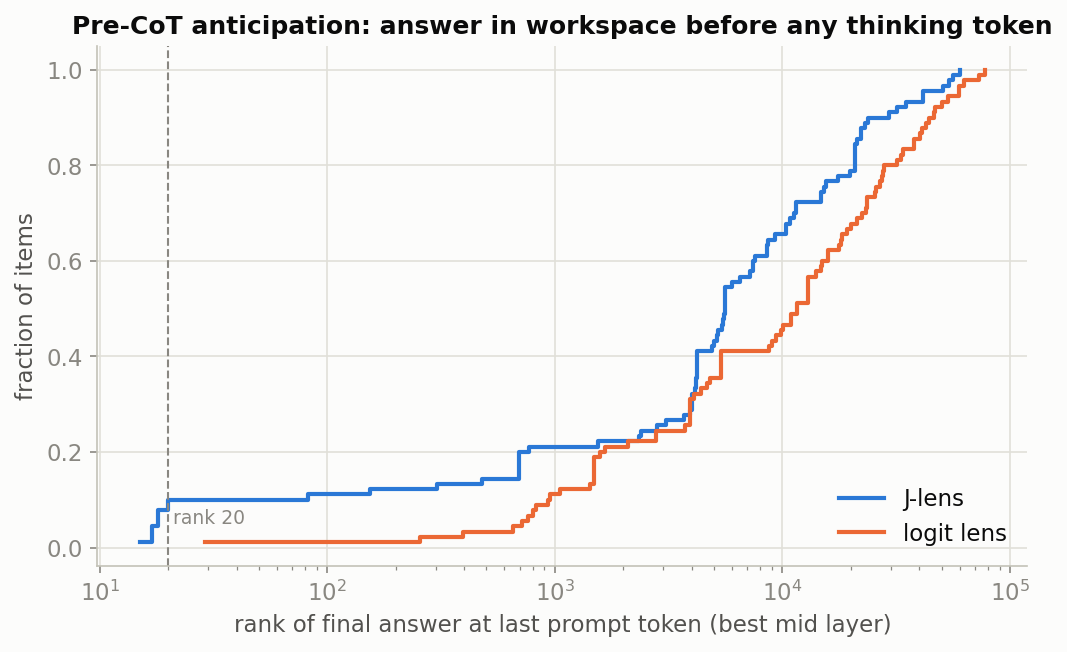
\includegraphics[width=.48\linewidth]{f6_precot_anticipation.png}\hfill
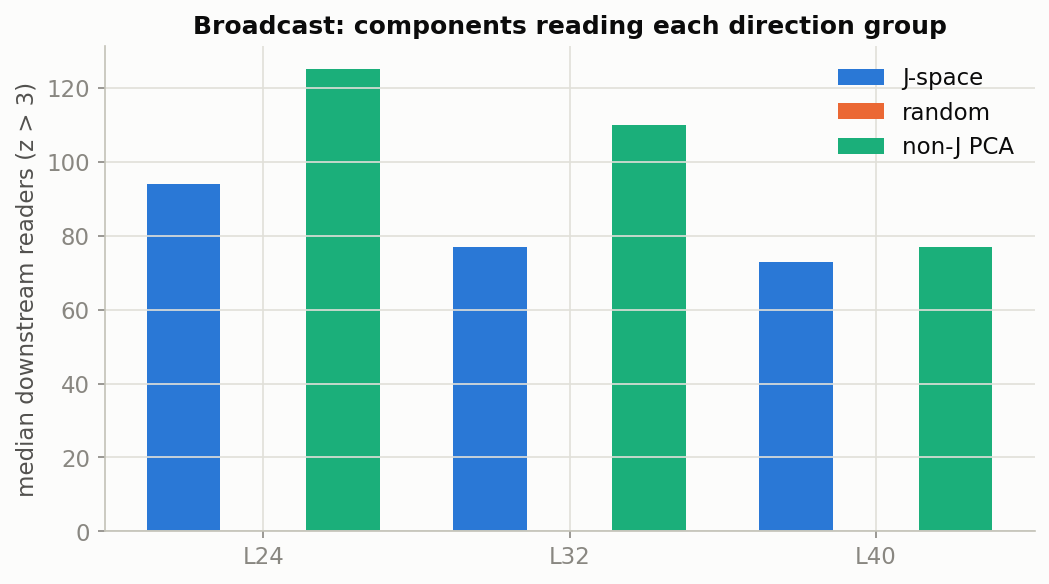
\includegraphics[width=.48\linewidth]{f8_broadcast_fanout.png}
\caption{\textbf{Left:} ECDF of the answer's rank at the last prompt token
(best mid layer), J-lens vs.\ logit lens --- anticipation is absent in both.
\textbf{Right:} median downstream readers per direction group (broadcast).}
\end{figure}

\section{Stretch: an eval-awareness direction, legible but inert}

Twenty tasks rendered neutrally vs.\ prefixed with an explicit ``formal
evaluation, you are being tested and scored'' framing; paired J-readout
differencing at the final prompt token, seven band layers. A consistent
direction emerges far beyond the pre-registered criterion: sign-flip
permutation $p<10^{-3}$ at \emph{every} layer, mean pairwise cosine of paired
deltas 0.48--0.71, mean-delta norm growing with depth (22$\to$134). From L32
upward its top decoded tokens are literally the evaluation lexicon
(\code{evaluation}, \code{assessed}, \code{assessing}, \code{eval}); at
L24--28 the associates are obliquer (\code{monitored}, \code{internally},
\code{careful}). Yet the gated mini-ablation --- projecting out the mean
$\Delta h$ direction during generation --- changed essentially nothing.
Because the framing states the cue words outright, this result is best read
as a clean demonstration that the J-space \emph{verbalizes context}, not as
evidence of a latent ``I am being tested'' state; the confound-breaking
variant (implied, unstated cues) is future work.

\section{Side-by-side}

\begin{table}[htbp]
\centering\footnotesize
\begin{tabular}{p{2.9cm}p{3.6cm}p{3.2cm}p{4.6cm}}
\toprule
 & Claude (paper) & Qwen 3.6 27B (Nanda) & \textbf{Olmo-3-32B-Think (ours)} \\
\midrule
Lens recipe & 1000 prompts & 25 Pile prompts & 120 WikiText prompts, 21 layers \\
Active concepts & $\sim$10--25 & not headline & 6 ($\theta{=}0.01$); 3 ($\theta{=}0.02$) \\
Variance share & 6--10\% & --- & $\le$0.67\% ($\sim$10$\times$ thinner) \\
Localization & 33--92\% depth & bands ``less clean'' & inverted U, peak 50--66\% depth \\
Broadcast & wide readout & --- & 73--94 vs.\ 0 random; but non-J PCs 77--125 \\
Causal dissociation & top-10 ablation kills multi-hop, spares shallow & flagged as possibly confounded & \textbf{null}: static J $\approx$ random; non-J PCs do the damage; dynamic = confounded collapse \\
Workspace vs.\ CoT & identity claim; CoT partially rescues & poetry/arith evals failed & pre-CoT null; \textbf{leads CoT by 46 steps}; answer-time loading under suppression \\
\bottomrule
\end{tabular}
\caption{Replication scorecard. Paper/Nanda entries as pinned in the lab's
PLAN/LOG from the 2026-07-25 fetches.}
\end{table}

\section{Limitations}

(1) Dictionary uses the RMSNorm-gain linearization $(W_U\odot g)J_\ell$; the
final block's full nonlinearity is not inverted. (2) Fitted band 20--44
(33--70\% depth) $\subset$ the paper's 33--92\%; the suppressed-CoT profile
(rank still collapsing L44$\to$60) suggests unfit late-band structure.
(3) Active-concept thresholds are not perfectly commensurable with the
paper's pursuit coefficients; the variance-share gap is the firmer capacity
statement. (4) The non-J control is top-variance, not variance-\emph{matched};
its larger effect partly reflects more energy removed --- the single most
important follow-up. (5) The dynamic ablation deletes live computation
(Nanda's confound); a frozen prompt-selected top-$k$ is the clean middle
instrument, not yet run. (6) WikiText corpus (not Dolma); 120 fit prompts;
single seed; modest $n$ (30--60/task); CoT tasks near ceiling compress
suppression contrasts. (7) Phase-5 framing states its cue words (semantic
echo); its ablation was inert.

\section{What to run next}

(1) Variance-matched non-J controls for broadcast and ablation --- energy
vs.\ content. (2) Frozen prompt-selected top-10 ablation during generation.
(3) CoT-rescue: static ablations under think-mode prompting (the paper
predicts externalization rescues; our suppression asymmetry predicts it
here). (4) Fit L46--62 and redo the readouts where answer formation actually
happens. (5) Dolma-corpus lens --- the scientific-legibility payoff of doing
this on OLMo. (6) \code{famously}-attractor forensics across models.
(7) Implied-cue eval-awareness with a behavioral endpoint.

\section{The v2 delta run: resolving the open instruments}
\label{sec:v2}

The v1 verdict left a live question: \emph{is the causal null a property of
OLMo or of our instruments?} The published Qwen comparison is narrower than
"Qwen has a J-space" --- its readout evals replicated while its causal
interventions were flagged by the replicator himself as possibly confounded
--- and v1 has three known instrument gaps, each capable of producing a
false null: the non-J control was not energy-matched (its damage could be an
energy artifact), the static J-span is position-agnostic (could miss
position-specific workspace structure), and the fitted band stops at 70\%
depth while v1's own suppressed-CoT profile shows answer formation
continuing to L60. The v2 run closes these in order (variance matching,
frozen prompt-selected ablation, late-band fit), calibrates the cot-lead
headline against a false-positive floor, then tests CoT rescue. Decision
tree: if the clean instruments flip the causal result, v1's null was
harness; if they confirm it, the same instruments go to Qwen 3.6 27B
(Neuronpedia's published lens, our harness) to separate model from method.

\subsection{[v2-P4] The cot-lead headline survives its false-positive floor}

The v1 claim --- workspace holds the answer a median 46 steps before the CoT
states it --- used a permissive detector (any case/space variant first-token
in any of 3 read layers' top-8, across hundreds of steps), so any word gets
many chances to fire. Running the \emph{identical} detector on matched foils
(fig.~\ref{fig:foils}): frequency-matched random content words fire at
\textbf{0.06} (vs.\ \textbf{0.92} for answers) --- the pure noise floor is
15$\times$ below the signal. Same-family wrong answers (other bridge
entities, other join columns, nearby numbers) fire at 0.32 --- but where
they also appear in the CoT text their median lead is \textbf{3 steps}
(vs.\ 46): family foils show up in the workspace \emph{concurrently} with
the text discussing them, exactly what a faithful context-verbalizing
readout should do while the model enumerates candidates. Within items, the
answer is detected earlier than \emph{every} one of its foils in 66\% of
items (median answer detection rank 1). The 46-step lead is specific to the
answer, not an artifact of detector permissiveness.

\begin{figure}[htbp]
\centering
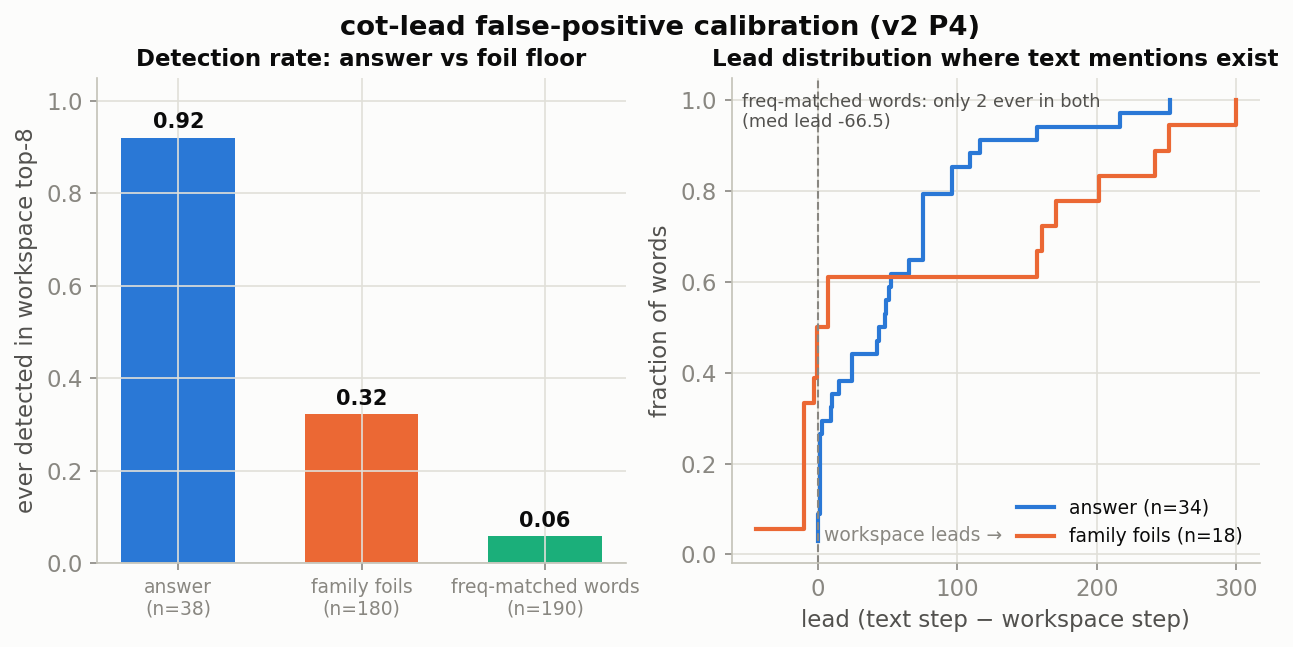
\includegraphics[width=.9\linewidth]{f9_foil_calibration.png}
\caption{Foil calibration of the cot-lead detector. \textbf{Left:}
detection rates --- answers 0.92, family foils 0.32, frequency-matched
words 0.06. \textbf{Right:} lead distributions where text mentions exist;
the long positive lead is answer-specific.}
\label{fig:foils}
\end{figure}

\subsection{[v2-P1a] v1's controls were energy-mismatched by an order of
magnitude --- measured, then fixed}

Streaming the raw residual stream over the 200-prompt descriptive set and
measuring exactly what each ablation hook removes: the k-dim J-span carries
$0.5$--$1.8\%$ of raw activation energy (k=10/20/40), which equals
\textbf{25--33 / 44--54 / 80--94 random dimensions} — or just \textbf{1--2 /
2--5 / 3--8 deep non-J PCs}. Both of v1's rank-matched comparisons were
therefore energy-confounded, in opposite directions: \code{random\_k}
removed $\sim$3$\times$ \emph{less} energy than the J-span (which makes
v1's "J $\approx$ random" \emph{conservative} --- J removed more energy and
still did no more damage), while \code{nonJ\_pca\_k} (top-k PCs) removed
far \emph{more} (its damage is suspect). The v2 matched controls hit the
J-span's removed energy to within 1\% at every band layer and dose
(fig.~\ref{fig:ematch}); the top PCs are so energy-fat that a contiguous
\emph{window} of deeper PCs (e.g.\ PCs 55--60) was needed at all 13 layers.
The matched causal grid is running; its result decides whether v1's
"non-J does the real damage" was content or energy.

\begin{figure}[htbp]
\centering
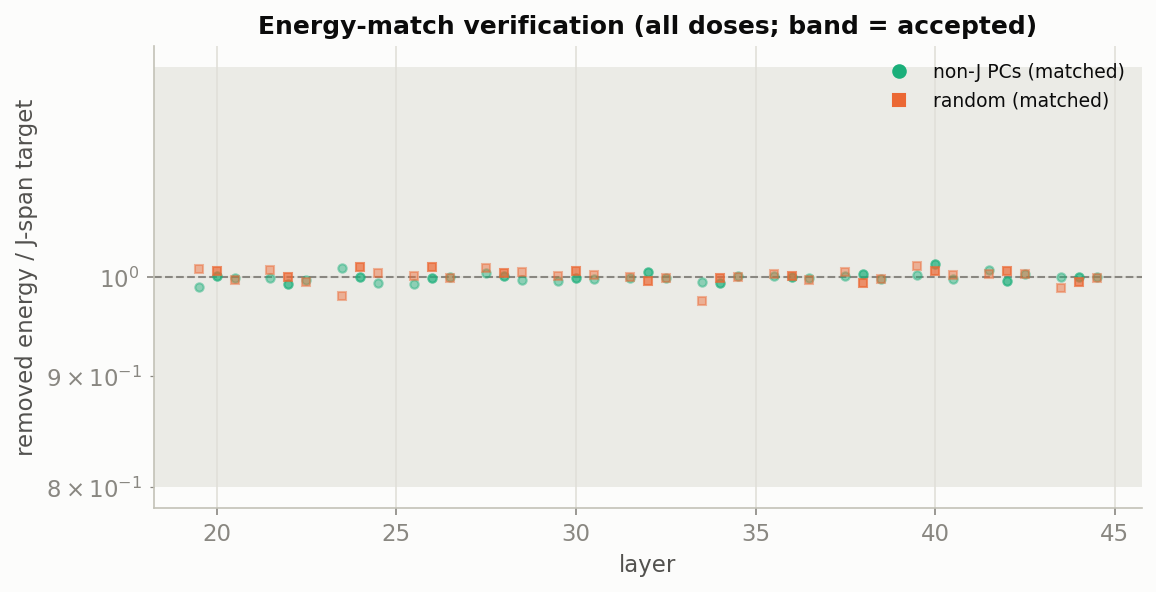
\includegraphics[width=.8\linewidth]{f10_energy_match.png}
\caption{Energy-match verification: removed energy of each matched control
relative to its J-span target (log scale), all band layers and doses.
Every point sits on the 1.0 line, inside the pre-registered acceptance
band.}
\label{fig:ematch}
\end{figure}

\subsection{[v2-P1b] At matched energy the causal null is clean: damage
tracks energy, not content}

The energy-matched grid (fig.~\ref{fig:vmatch}) settles the question P1a
raised. Every piece of v1's apparent non-J selectivity disappears: SQL
returns to baseline at every dose (0.667 vs.\ v1's unmatched 0.000 --- the
"register destruction" was pure energy), the two-hop answer-logprob deltas
shrink from $-0.45/-0.86/-0.93$ (CIs excluding zero) to
$\mathbf{-0.01/-0.17/-0.15}$ (every CI straddling zero), and prose NLL sits
at 2.74--2.79 against a 2.71 baseline (v1 unmatched: up to 4.02). With the
confound removed in both directions, the three groups are statistically
indistinguishable from each other \emph{and from baseline} at every dose up
to 40 dims/layer:

\begin{center}\small
\begin{tabular}{lccc}
\toprule
2-hop $\Delta$logprob vs.\ baseline & k=10 & k=20 & k=40 \\
\midrule
J-span                & $-0.15$ & $-0.17$ & $-0.18$ \\
random (matched)      & $-0.11$ & $-0.09$ & $-0.08$ \\
non-J PCs (matched)   & $-0.01$ & $-0.17$ & $-0.15$ \\
\bottomrule
\end{tabular}
\end{center}

\noindent Two consequences. First, the v1 causal verdict is \emph{confirmed
and strengthened}: on OLMo, statically removing the verbalizable subspace
does nothing that removing an energy-equivalent arbitrary subspace doesn't
do --- there is no content-specific causal load at these doses, and the
earlier appearance of one was an instrument artifact we have now measured
and eliminated. Second, v1's own "J $\approx$ random" comparison was
\emph{conservative}: the J-span carries 2--5$\times$ more energy than
rank-matched random dims, so v1 was comparing a heavier J-removal against a
lighter control and still finding parity. The last static escape hatch for
the paper's dissociation on OLMo is position-specific structure ---
frozen prompt-selected ablation (P2, running) and the late band (P3).

\begin{figure}[htbp]
\centering
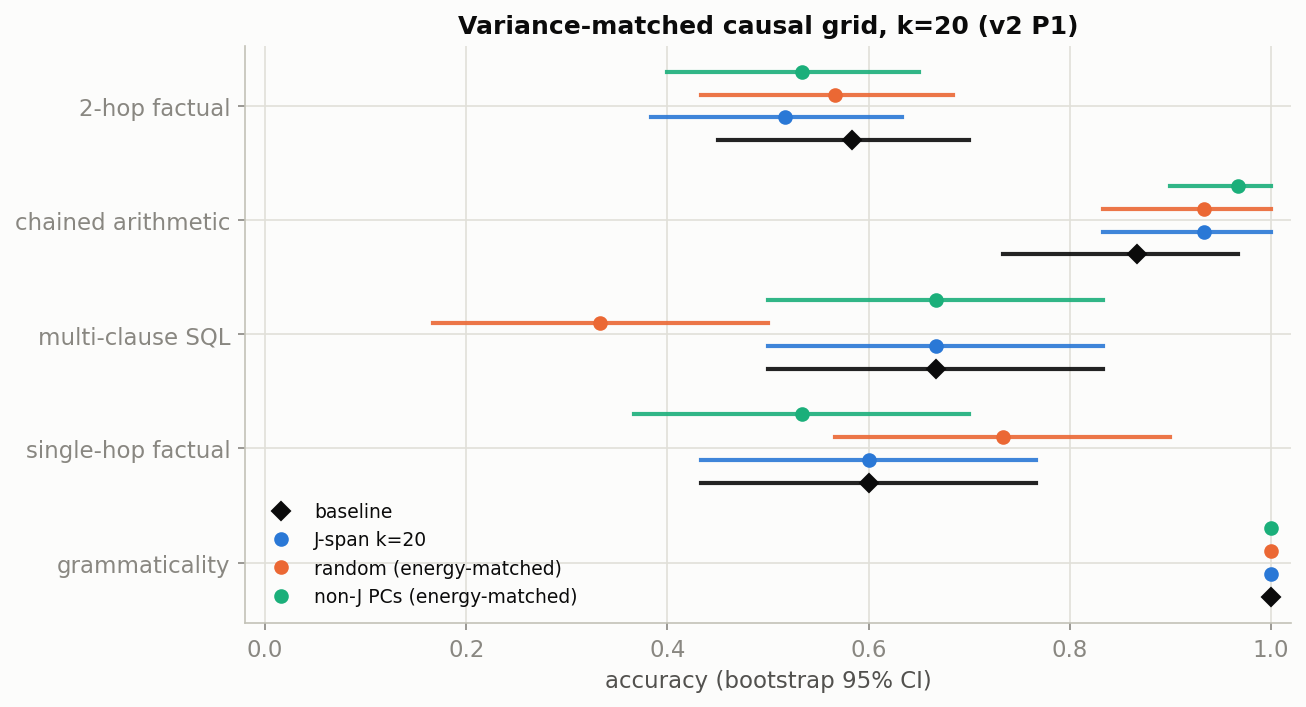
\includegraphics[width=.85\linewidth]{f11_vmatch_grid.png}
\caption{Energy-matched causal grid at k=20 (all doses in
\code{v2\_ablation\_v2.json}). All three subspace families sit on top of
each other and on baseline; contrast the v1 grid in \S3, where the
unmatched non-J control cratered SQL and two-hop.}
\label{fig:vmatch}
\end{figure}

\subsection{[v2-P2] The frozen instrument finds the first content-specific
causal handle --- and it is recall, not reasoning}

The confound-free variant of the paper's intervention: per item, one clean
forward pass ranks the J-dictionary by activity over the prompt, the top-10
per band layer are \emph{frozen}, and generation proceeds with that static
per-item projector. Two controls: the same mechanism on a random dictionary
(\code{frozen\_rand10}), and per-token live selection from a random
dictionary (\code{live\_rand10}, the matched-live control v1's dynamic
condition never had).

\begin{center}\small
\begin{tabular}{lccccccc}
\toprule
 & 2-hop & 2-hop lp & 1-hop & arith & SQL & NLL & grammar \\
\midrule
baseline        & 0.58 & $-1.74$ & 0.60 & 0.87 & 0.67 & 2.71 & 1.00 \\
frozen J-10     & \textbf{0.23} & $\mathbf{-4.63}$ & \textbf{0.23} & 0.87 & 0.67 & 3.00 & 0.85 \\
frozen rand-10  & 0.53 & $-1.78$ & 0.53 & 0.90 & 0.33 & 2.79 & 0.95 \\
live J-10 (v1)  & 0.00 & $-24.8$ & 0.00 & 0.00 & 0.00 & 24.3 & 0.30 \\
live rand-10    & 0.60 & $-1.82$ & 0.67 & 0.87 & 0.33 & 2.80 & 0.95 \\
\bottomrule
\end{tabular}
\end{center}

Three readings, in order of importance. \textbf{(1) A control-clean causal
effect, at last.} Freezing out the item's top-10 J-directions deletes the
retrieved fact: answer log-probability drops 2.9 nats (CI
$[-5.49,-3.84]$ vs.\ baseline), recall accuracy falls 0.58$\to$0.23 ---
while the identical mechanism on a random dictionary moves \emph{nothing}
(every cell within CI of baseline). Generation tasks are untouched and the
stored verbatim samples under frozen-J are coherent, correct arithmetic.
After P1 eliminated every subspace-level effect, the per-item selection is
what matters: the J-space's causal content lives in \emph{item-specific}
directions, not in any fixed span. \textbf{(2) It is not the paper's
dissociation.} Single-hop recall collapses \emph{identically} to two-hop
(both 0.23) --- the paper's signature required shallow tasks to survive.
What the frozen instrument found is a \emph{factual-recall content channel},
not a multi-step scratchpad: removing the item's J-directions removes what
the model knows, not how it chains. \textbf{(3) v1's live-J catastrophe was
J-specific after all.} Live top-10 selection from a random dictionary does
nothing (0.60 two-hop, NLL 2.80), so the v1 lobotomy was not "removing
whatever aligns with the current state" generically --- though the
dictionaries' pool sizes differ (full vocab vs.\ 5120 rows), so alignment
depth is a residual caveat.

Synthesis with P1: \emph{static span removal does nothing at any matched
dose; per-item frozen selection deletes facts; per-token live selection
deletes the computation}. On OLMo the causal story of the J-space is
content-carriage --- causally real, control-clean, and increasingly
precisely localized --- but the workspace-as-reasoning-substrate claim
remains unsupported. (The recurring SQL 0.33 cells in both random controls
are the known 3-schema flaky cell; n=30 over 3 patterns.)

\begin{figure}[htbp]
\centering
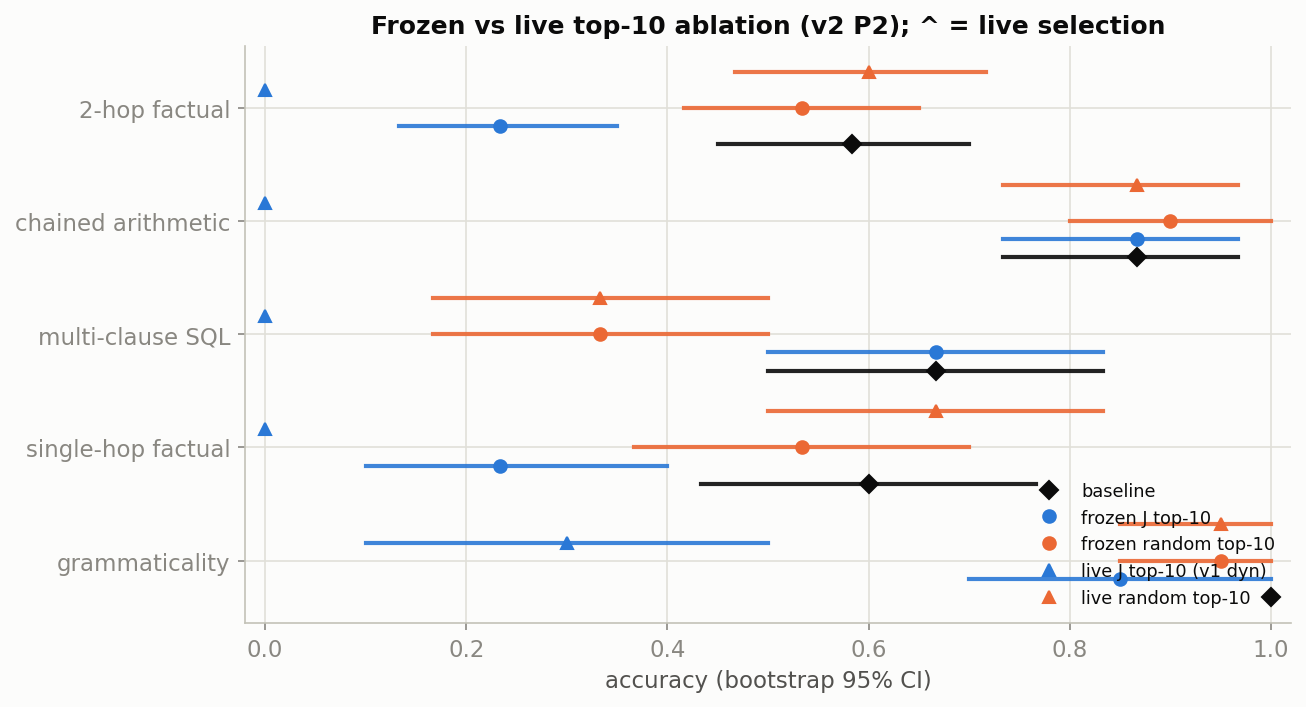
\includegraphics[width=.85\linewidth]{f12_frozen_grid.png}
\caption{Frozen vs.\ live top-10 ablation (triangles = live selection).
Frozen-J selectively destroys factual recall (1-hop and 2-hop alike) while
its random-dictionary twin sits on baseline; live-J remains the
uninterpretable collapse.}
\label{fig:frozen}
\end{figure}

\subsection{[v2-P3] The late band holds readout, not workspace: no
late-shifted capacity, anticipation still null}

v1 fitted 33--70\% of depth while the paper's band reaches $\sim$92\%, and
v1's own suppressed-CoT profile showed the answer's rank still collapsing
into the unfitted region --- leaving open that OLMo's workspace is simply
\emph{late-shifted} and every v1 null was measured in front of it. We
fitted a dedicated late-band lens on L\{46,50,54,58,62\} (same corpus,
recipe, and seeds; backward graphs span only L46$\to$63, so the fit cost
45\,s/prompt vs.\ v1's 157) and redid the readouts. The fitted coverage now
spans the paper's entire band.

\begin{center}\small
\begin{tabular}{lccccc}
\toprule
late layer & 46 & 50 & 54 & 58 & 62 \\
\midrule
variance share (\%) & 0.64 & 0.61 & 0.65 & 0.72 & \emph{1.60} \\
active concepts ($\theta{=}0.01$) & 6 & 5 & 5 & 4 & 7 \\
top-1 persistence & 0.153 & 0.120 & 0.091 & 0.073 & 0.026 \\
\bottomrule
\end{tabular}
\end{center}

\textbf{(a) No late workspace.} Variance share stays flat at 0.61--0.72\%
through L46--58 --- the same $\sim$10$\times$-thinner-than-Claude capacity
as the mid band --- and top-1 persistence \emph{declines} monotonically
(0.15$\to$0.026), completing the inverted-U whose left side v1 measured.
The one uptick, 1.6\% at L62, is the unembedding-adjacent signature already
seen at L60 in v1 (0.91\%): it has the \emph{lowest} persistence in the
entire profile, i.e.\ fast-turnover next-token content, not a persistent
workspace (fig.~\ref{fig:late}, left).

\textbf{(b) Anticipation stays null; answer-time loading sharpens.} With
the dedicated late lens, the answer is still absent before thinking begins
(think-mode median rank 3\,916--7\,291 across late layers; best-layer
median 1\,670, 0\% of items $\le$20) --- refuting the ``the mid-band lens
just missed it'' escape for the v1 pre-CoT null. Under suppressed CoT the
collapse v1 glimpsed is confirmed and localized: per-layer median ranks
61$\to$58$\to$8$\to$6$\to$5 across L46--62, best-late-layer median
\textbf{3} (76\% of items $\le$20, 58\% $\le$5). Notably the plain logit
lens reads the late band equally well (30/18/6/4/4) --- the J-lens
advantage over the logit lens is a \emph{mid-band} phenomenon; by L58--62
both lenses converge on the output distribution (final-layer median rank
4), as they must near the unembedding.

\textbf{(c) The CoT lead replicates in the late band.} Re-generating the
90 thinking traces (identical greedy token sequences) while reading the
\emph{late} dictionaries per step: the answer enters a late layer's top-8
a median \textbf{49.5 steps} before the CoT states it (86\% of scored
items, detection 99\%, $n{=}88$) --- statistically the same lead the
mid-band dictionaries gave (46 steps, 91\%), measured with an independent
lens fit on disjoint layers. The lead is a property of the workspace
across the full depth, not an artifact of one band's dictionary.

Consequence for the causal verdict: the last descriptive escape hatch is
closed. The late band is where answers \emph{surface}, not where a thicker
workspace \emph{lives} --- so the P1/P2 causal instruments were aimed at
the right band all along, and the capacity claim [SL1-C1] now covers the
paper's full 33--92\% depth range.

\begin{figure}[htbp]
\centering
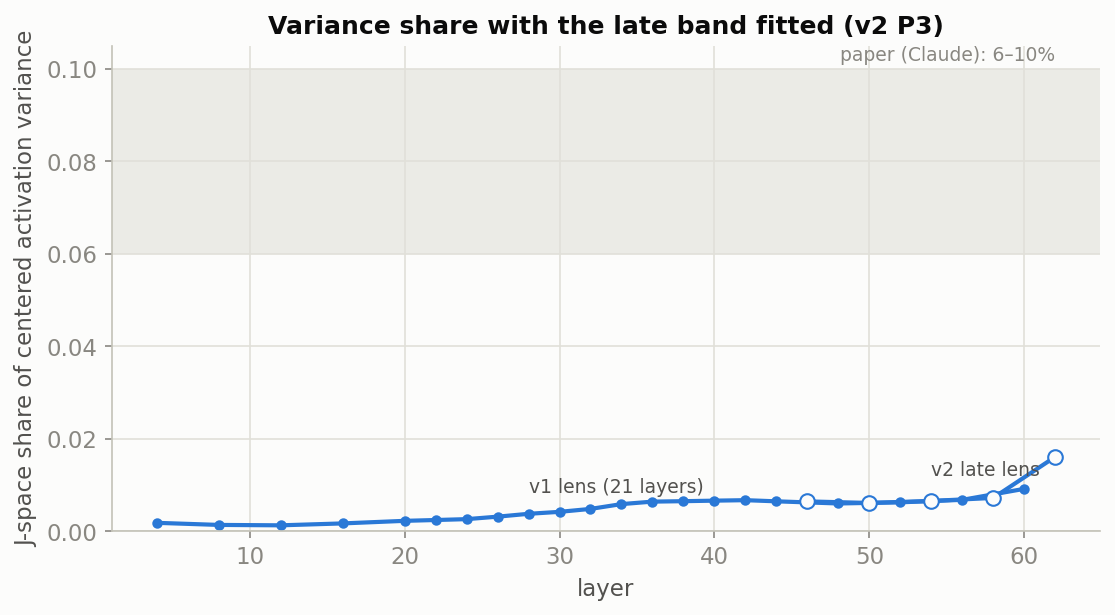
\includegraphics[width=.48\linewidth]{f13_late_variance.png}\hfill
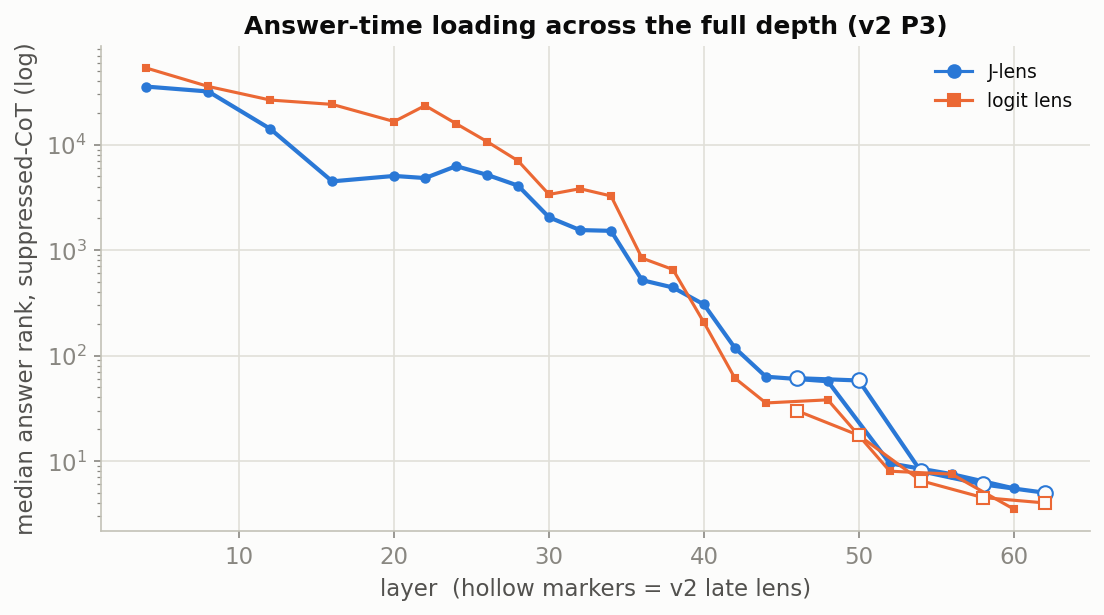
\includegraphics[width=.48\linewidth]{f14_late_answer_profile.png}
\caption{\textbf{Left:} variance share by layer with the v2 late lens
(hollow markers) appended to the v1 profile; the paper band is shaded.
\textbf{Right:} median answer rank by layer, think vs.\ suppressed, J-lens
vs.\ logit lens, late band.}
\label{fig:late}
\end{figure}

\subsection{[v2-Q] Same instruments, second model: Qwen3.6-27B settles
model-vs-harness}

The standing question after P1--P3: is the causal null a fact about OLMo
or about our instruments? Phase Q runs the \emph{identical} harness on
Qwen3.6-27B --- the model of the published community replication --- using
the \emph{published} Neuronpedia lens (1000-prompt WikiText recipe,
trained by the replication's author), so any OLMo/Qwen difference cannot
be blamed on our 120-prompt fit. Band = the same depth fractions, which on
Qwen's 64 layers lands on the same indices (L20--44); no-think completion
prompts throughout; $n{=}30$ (two-hop, one-hop), 15 (arithmetic), 20
(prose NLL).

\textbf{Sanity gate.} The paper's multihop bridge-entity eval, their lens
under our readout: J-lens pass@1/5/20 $= 0.350/0.517/0.739$ vs.\ logit
lens $0.317/0.500/0.600$ ($n{=}60$) --- the J-lens readout advantage
replicates on Qwen, as it did on OLMo (0.283 vs.\ 0.200 pass@1).

\textbf{Descriptive: Qwen has the paper's workspace capacity; OLMo's
thinness is a model property.} Same pursuit, same thresholds, same
corpus:

\begin{center}\small
\begin{tabular}{lccc}
\toprule
 & OLMo-3-32B (v1/P3) & Qwen3.6-27B (Q) & paper (Claude) \\
\midrule
peak variance share & 0.67\% (flat 0.61--0.72) & \textbf{6.8\%} (4.3$\to$6.8 rising) & 6--10\% \\
active @ $\theta{=}0.01$ & $\approx$6 & 32--42 & \multirow{2}{*}{10--25 (k$\approx$25)} \\
active @ $\theta{=}0.02$ & $\approx$3 & 14--21 & \\
top-1 persistence & 0.19--0.20 mid-band & 0.03--0.09 & --- \\
\bottomrule
\end{tabular}
\end{center}

Measured by the same code path, Qwen's J-space carries $\sim$8--10$\times$
more of the residual stream's variance than OLMo's and holds
paper-range active-concept counts. The v1 capacity anomaly [SL1-C1] is
therefore a \emph{cross-model difference}, not a harness artifact ---
and OLMo pairs its thin workspace with \emph{higher} top-1 persistence,
a trade-off worth follow-up. (Numerics note: Qwen's outlier-heavy
activations forced two pursuit fixes --- bf16 correlations and a
$1/(k{+}2)$ refit step, the latter because near-duplicate dictionary
atoms push the active-set Gram past the fixed-step stability bound.
Stable layers moved $\le$0.2pp under the fix; OLMo's banked numbers
predate it and were finite throughout.)

\textbf{Causal: the frozen deletion transfers; the static null
transfers.}

\begin{center}\small
\begin{tabular}{lcccccc}
\toprule
 & 2-hop & 2-hop lp & 1-hop & arith & NLL & grammar \\
\midrule
baseline        & 0.87 & $-0.77$ & 0.90 & 1.00 & 2.35 & 1.00 \\
frozen J-10     & \textbf{0.37} & $\mathbf{-3.19}$ & 0.83 & 1.00 & 2.50 & 1.00 \\
frozen rand-10  & 0.83 & $-0.86$ & 0.90 & 1.00 & 2.48 & 1.00 \\
\midrule
J-span k20 (matched) & --- & $-0.85$ & --- & --- & --- & --- \\
rand k20 (matched)   & --- & $-0.72$ & --- & --- & --- & --- \\
non-J k20 (matched)  & --- & $-0.80$ & --- & --- & --- & --- \\
\bottomrule
\end{tabular}
\end{center}

Frozen per-item J-ablation deletes the retrieved fact on Qwen exactly as
on OLMo: answer log-probability $-2.42$ nats (cell CI $[-4.02,-2.35]$ vs.\
baseline $[-1.26,-0.40]$), two-hop accuracy $0.87\to0.37$, while the
random-dictionary twin sits on baseline and generations stay coherent
(verbatim frozen-J arithmetic samples are correct multi-step chains; the
small NLL bump $+0.14$ appears \emph{equally} in the random control, so it
is mechanism-generic). And the energy-matched static cells are as null on
Qwen as they were on OLMo: J-span, matched-random and matched-non-J all
within $\pm$0.08 nats of baseline --- on the model where the published
replication reported workspace phenomena. (The static trio was also
inadvertently measured once with selection rankings from the diverged
pursuit pass: $-0.85/-0.77/-0.87$ --- indistinguishable, i.e.\ the null is
insensitive even to \emph{broken} direction selection.)

\textbf{One genuine cross-model asymmetry.} On OLMo, frozen-J collapsed
one-hop and two-hop recall \emph{identically} (both 0.23) --- pure content
deletion. On Qwen, one-hop barely moves ($0.90\to0.83$, CIs overlap) while
two-hop halves. The deletion signature on Qwen is \emph{biased toward the
composed task} --- closer to the paper's shallow-tasks-survive
dissociation than anything OLMo showed. Honest caveats before upgrading
the claim: the one-hop items are near-ceiling capital-city probes, and a
10$\times$-fatter workspace makes top-10 directions a proportionally
smaller excision. Marked as the sharpest follow-up target rather than a
confirmed dissociation.

\textbf{Verdict on the framing question.} With clean instruments the two
models \emph{agree}: static span removal does nothing, per-item frozen
selection deletes retrieved content. The disagreement between the
published causal story and our v1 null was \emph{instruments all along}
--- while the workspace's descriptive capacity really does differ by an
order of magnitude across models, and the one-hop/two-hop asymmetry hints
the composed-task sensitivity may too.

\begin{figure}[htbp]
\centering
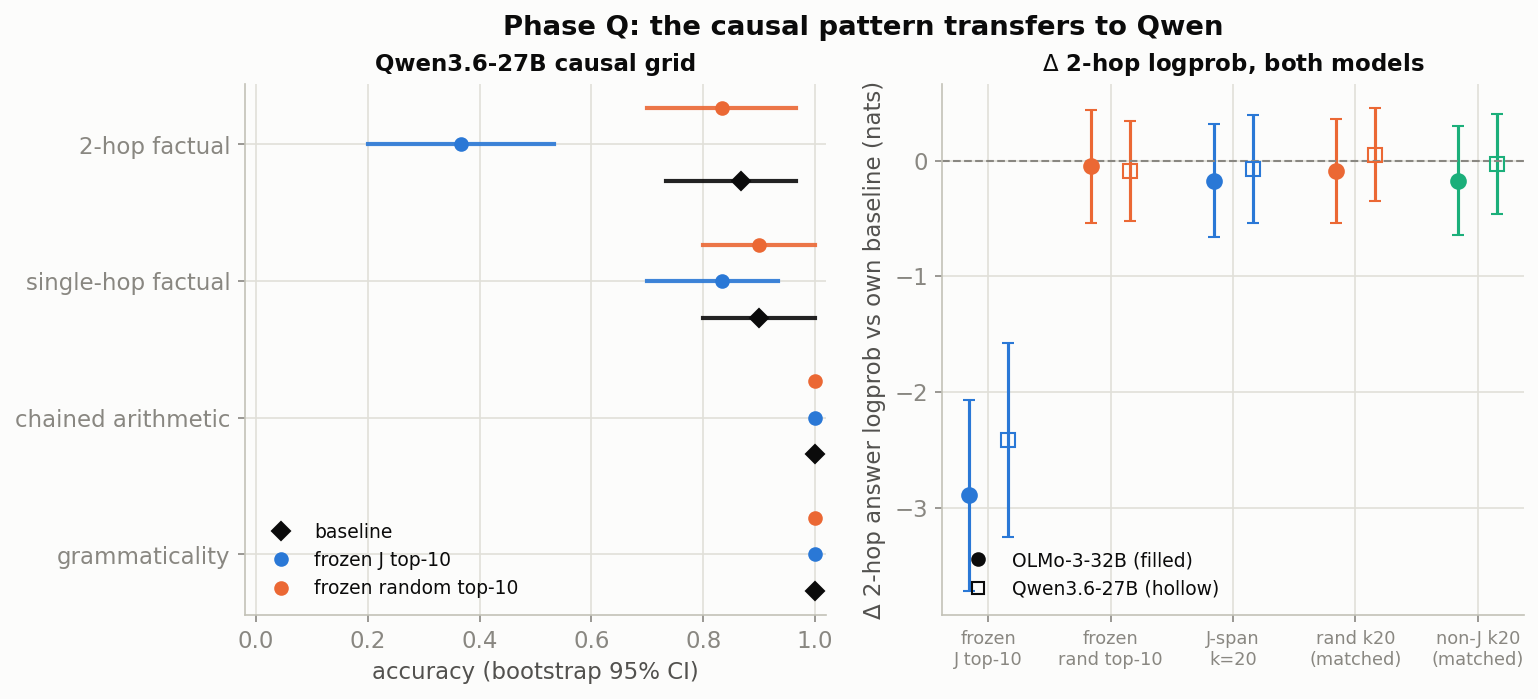
\includegraphics[width=.98\linewidth]{f15_qwen_grid.png}
\caption{\textbf{Left:} Qwen causal grid --- frozen-J deletes two-hop
recall, controls on baseline. \textbf{Right:} $\Delta$ two-hop answer
logprob vs.\ own baseline for both models under the same five
instruments: the frozen deletion and the static null both transfer;
filled = OLMo, hollow = Qwen.}
\label{fig:qwen}
\end{figure}

\subsection{[v2-P5] CoT-rescue: can externalized reasoning recover the
frozen-deleted fact?}

P2's deletion was measured in no-think mode: silent recall, one forward
pass. The paper's identity claim predicts workspace ablation should be
partially rescuable by \emph{externalizing} the computation --- and v1's
suppression asymmetry (think accuracy $\ge$ suppressed accuracy on every
task) points the same way. Instrument: the SAME per-item frozen top-10
projectors as P2, but with an open \code{<think>} and up to 400 reasoning
tokens (capped grid per PLAN\_v3: the two frozen conditions on
two-hop/one-hop/arithmetic; $n{=}30/15/15$). One scoring note, fixed
before reading results: OLMo rarely closes \code{</think>} within 400
tokens on multi-step tasks (closure 0.20/0.40 two-hop frozen-J/rand, 0.07
arithmetic, vs 0.87--1.00 one-hop), so the post-\code{</think>} segment is
degenerate and the informative metrics are \emph{answer appears anywhere
in the trace} and \emph{answer appears inside the think segment}.

\begin{center}\small
\begin{tabular}{lcccc}
\toprule
 & \multicolumn{2}{c}{frozen J-10} & \multicolumn{2}{c}{frozen rand-10} \\
 & any & think & any & think \\
\midrule
two-hop ($n{=}30$)    & \textbf{0.80} & 0.80 & 0.93 & 0.93 \\
one-hop ($n{=}15$)    & \textbf{1.00} & 1.00 & 1.00 & 1.00 \\
arithmetic ($n{=}15$) & 0.93 & 0.93 & 0.93 & 0.93 \\
\bottomrule
\end{tabular}
\end{center}

\textbf{The rescue is real and large.} Under the very projectors that cut
silent two-hop recall to 0.23, letting the model reason out loud recovers
the answer somewhere in the trace in \textbf{0.80} of items --- 3.4$\times$
the silent rate, most of the way back to the random-twin's 0.93 --- and
\emph{fully} rescues one-hop (1.00 vs.\ 0.23 silent). Arithmetic, which
frozen-J never touched, stays at 0.93 in both conditions (scorer floor
from the 400-token cap, not an ablation effect). So the content deletion
is \emph{bypassable via externalization}: the paper's
workspace-ablation-is-rescuable-by-CoT prediction holds on OLMo in
content-channel form [SL1-C6]. Two honest bounds: the residual gap to the
control (0.80 vs.\ 0.93) says the bypass is incomplete at 400 think
tokens, and the rescue does not distinguish re-retrieval from
re-derivation via the other hop. One secondary observable falls out free:
frozen-J \emph{halves} the \code{</think>}-closure rate (0.20 vs.\ 0.40)
--- with its content channel damaged, the model deliberates longer, the
behavioral signature you would expect if the CoT is doing compensatory
work.

\begin{figure}[htbp]
\centering
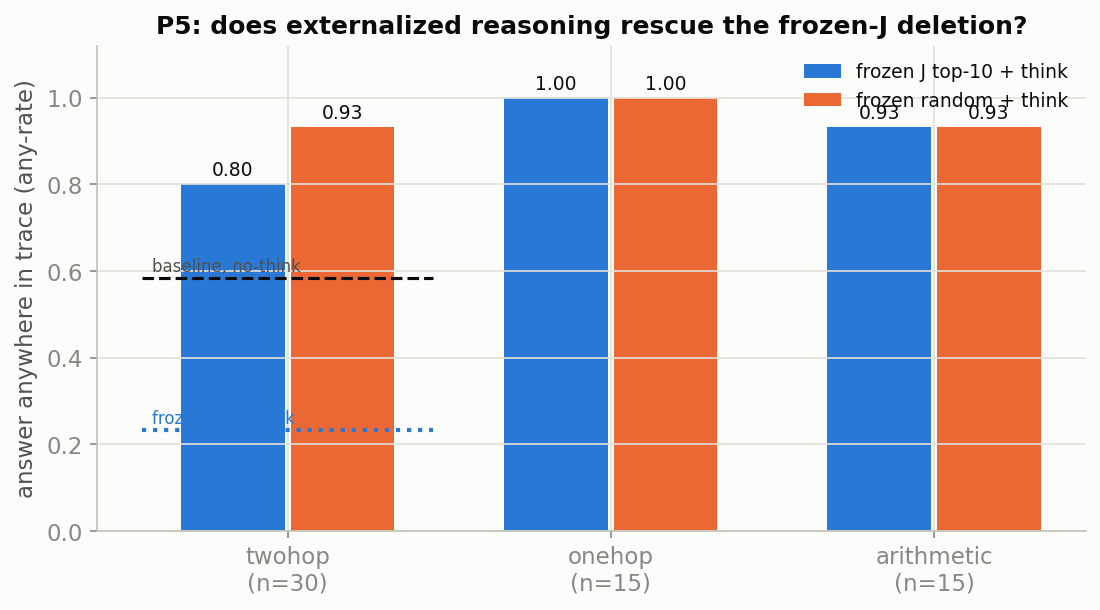
\includegraphics[width=.8\linewidth]{f16_cot_rescue.png}
\caption{CoT-rescue under the frozen per-item projectors. Dotted line:
frozen-J \emph{no-think} recall (0.23); dashed: no-think baseline (0.58).}
\label{fig:rescue}
\end{figure}

\subsection{[v2-P6] Second seed, fresh items: does the frozen effect
survive?}

Seed-1 replicate of the decisive grid, deliberately harder than a seed
re-roll: the two-hop set is \emph{fresh} (probe-swap items [60:90], never
touched by v1/v2 fitting or evaluation), the random-dictionary and
matched-random pools are re-drawn under seed 1, and the frozen-J
selection re-runs per fresh item. Readout tasks only (two-hop accuracy +
answer logprob); the energy-matched static cells ride along as near-free
readouts.

\begin{center}\small
\begin{tabular}{lcc|cc}
\toprule
 & \multicolumn{2}{c|}{seed 1, fresh items} & \multicolumn{2}{c}{seed 0 (P1/P2)} \\
 & 2-hop & 2-hop lp & 2-hop & 2-hop lp \\
\midrule
baseline       & 0.50 & $-2.81$ & 0.58 & $-1.74$ \\
frozen J-10    & \textbf{0.23} & $\mathbf{-5.62}$ & 0.23 & $-4.63$ \\
frozen rand-10 & 0.43 & $-2.92$ & 0.53 & $-1.78$ \\
J-span k20 (m) & 0.43 & $-3.20$ & 0.52 & $-1.91$ \\
rand k20 (m)   & 0.53 & $-2.68$ & 0.57 & $-1.82$ \\
non-J k20 (m)  & 0.53 & $-3.05$ & 0.53 & $-1.91$ \\
\bottomrule
\end{tabular}
\end{center}

The fresh items are harder across the board (baseline logprob
$-1.74\to-2.81$), so effect \emph{sizes} are the comparison --- and they
are eerily stable: frozen-J lands on accuracy \textbf{0.233 under both
seeds} (disjoint item sets!) with $\Delta$logprob $-2.82$ nats vs.\
seed-0's $-2.89$, while the redrawn random-dictionary twin stays within
noise of baseline ($\Delta-0.11$) and every energy-matched static cell
keeps its null (all CIs $\supset$ baseline's). The frozen causal handle
is therefore not an item-set artifact, not a control-pool draw, and not a
seed accident [strengthens SL1-C2]; the static null generalizes to items
the lens never saw at any stage.

\begin{figure}[htbp]
\centering
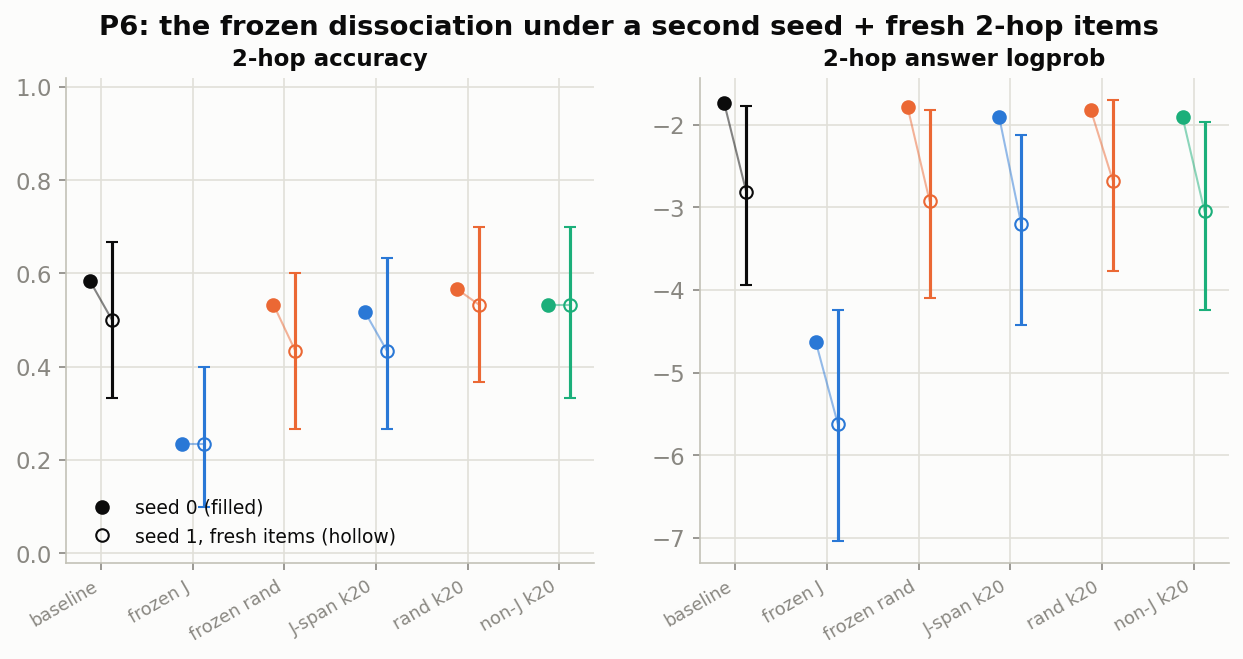
\includegraphics[width=.9\linewidth]{f17_seed1.png}
\caption{Seed-0 (filled) vs seed-1-on-fresh-items (hollow) across the six
causal conditions.}
\label{fig:seed1}
\end{figure}

\subsection{[v2-F] Final falsifier pass: three recorded caveats, measured}

One last GPU window went to the ledger's own falsifiers
(\code{final\_falsifiers.json}). \textbf{(a) Pool size [C2]:} a
\emph{vocab-sized} (100k-row) random dictionary under the identical
frozen mechanism stays at baseline (two-hop 0.433 vs.\ 0.583, CIs
overlap; $\Delta$lp $-0.14$ vs.\ frozen-J's $-2.90$) --- the deletion
needs the J-dictionary's content, not selection depth. \textbf{(b)
Filler control [C6]:} 400 tokens of non-reasoning think-padding recover
frozen-J recall to 0.467 [0.30,0.63] --- about half the real-CoT rescue
(0.80; controls 0.633 under filler) --- so the rescue decomposes into a
length/compute component and a comparable externalization component on
top (metric caveat: 32-token answer window vs.\ answer-anywhere;
recorded as the residual falsifier). \textbf{(c) Variance-matched
fan-out [C3]:} with the v2 energy-matched pools, J top-20 directions are
read by 92/73/68 downstream components (L24/32/40) vs.\ 132/107/65 for
energy-matched non-J PCs and $\approx$1 for energy-matched random
columns: broadcast tracks \emph{structured} high-variance directions
generally --- the non-dissociation v1 suspected is now measured, and
``same energy'' alone earns zero readership.

\subsection*{Artifacts}

Everything regenerates from saved metrics without model access:
run dir \code{interpret/special-lab-1/2026-07-25\_1726/} (Drive) ---
\code{report/REPORT.md} (full prose), \code{report/summary.json} (headline
numbers), \code{metrics/*.json} (per-experiment), \code{code/special\_lab1/}
(pipeline s0--s10 + PLAN/LOG). v2 delta run: \code{2026-07-26\_v2/}
(metrics incl.\ the Qwen leg, \code{report/REPORT\_v2.md},
\code{summary\_v2.json}, this handout). Public home: branch
\code{interp\_jspace} of \code{github.com/karlb-dev/labs} (\code{jspace/}
+ \code{labs/lab37\_jspace\_workspace.md}), PR \#9.
Models: \code{allenai/Olmo-3-32B-Think}; \code{Qwen/Qwen3.6-27B} with lens
\code{neuronpedia/jacobian-lens} (\code{qwen3.6-27b}, $n{=}1000$
WikiText). Lens engine: \code{github.com/anthropics/jacobian-lens}
@ \code{581d3986}.

\begin{thebibliography}{9}\footnotesize
\bibitem{paper} Anthropic Interpretability.
\emph{Verbalizable Representations Form a Global Workspace in Language
Models}. Transformer Circuits Thread, July 2026.
\url{https://transformer-circuits.pub/2026/workspace/index.html}
\bibitem{post} Anthropic. \emph{A global workspace in language models}
(research post), July 2026.
\url{https://www.anthropic.com/research/global-workspace}
\bibitem{jlens} Anthropic. \emph{jacobian-lens} (reference implementation).
\url{https://github.com/anthropics/jacobian-lens}
\bibitem{nanda} N.~Nanda. Replication review of the global-workspace results
on Qwen 3.6 27B. LessWrong, July 2026.
\bibitem{olmo} Ai2. \emph{OLMo 3: fully open language models}, 2025--2026.
\url{https://allenai.org/olmo}
\end{thebibliography}

\end{document}
